\documentclass[11pt]{article}
%DIF LATEXDIFF DIFFERENCE FILE
%DIF DEL Old\main_test.tex       Fri Mar 24 13:19:48 2023
%DIF ADD Current\main_test.tex   Fri Mar 24 13:19:49 2023
\usepackage{amsmath}
\usepackage{float}
\usepackage{amssymb}
\usepackage{graphicx}
\graphicspath{{figures/}}

\title{Magical Fish Are More Powerful Raw}
\date{2022\\ March}
\author{Matthew Luu \\ Magic Department\thanks{I am not magical} \and John Doe \\ Science Department}
%DIF PREAMBLE EXTENSION ADDED BY LATEXDIFF
%DIF UNDERLINE PREAMBLE %DIF PREAMBLE
\RequirePackage[normalem]{ulem} %DIF PREAMBLE
\RequirePackage{color}\definecolor{RED}{rgb}{1,0,0}\definecolor{BLUE}{rgb}{0,0,1} %DIF PREAMBLE
\providecommand{\DIFadd}[1]{{\protect\color{blue}\uwave{#1}}} %DIF PREAMBLE
\providecommand{\DIFdel}[1]{{\protect\color{red}\sout{#1}}}                      %DIF PREAMBLE
%DIF SAFE PREAMBLE %DIF PREAMBLE
\providecommand{\DIFaddbegin}{} %DIF PREAMBLE
\providecommand{\DIFaddend}{} %DIF PREAMBLE
\providecommand{\DIFdelbegin}{} %DIF PREAMBLE
\providecommand{\DIFdelend}{} %DIF PREAMBLE
\providecommand{\DIFmodbegin}{} %DIF PREAMBLE
\providecommand{\DIFmodend}{} %DIF PREAMBLE
%DIF FLOATSAFE PREAMBLE %DIF PREAMBLE
\providecommand{\DIFaddFL}[1]{\DIFadd{#1}} %DIF PREAMBLE
\providecommand{\DIFdelFL}[1]{\DIFdel{#1}} %DIF PREAMBLE
\providecommand{\DIFaddbeginFL}{} %DIF PREAMBLE
\providecommand{\DIFaddendFL}{} %DIF PREAMBLE
\providecommand{\DIFdelbeginFL}{} %DIF PREAMBLE
\providecommand{\DIFdelendFL}{} %DIF PREAMBLE
\newcommand{\DIFscaledelfig}{0.5}
%DIF HIGHLIGHTGRAPHICS PREAMBLE %DIF PREAMBLE
\RequirePackage{settobox} %DIF PREAMBLE
\RequirePackage{letltxmacro} %DIF PREAMBLE
\newsavebox{\DIFdelgraphicsbox} %DIF PREAMBLE
\newlength{\DIFdelgraphicswidth} %DIF PREAMBLE
\newlength{\DIFdelgraphicsheight} %DIF PREAMBLE
% store original definition of \includegraphics %DIF PREAMBLE
\LetLtxMacro{\DIFOincludegraphics}{\includegraphics} %DIF PREAMBLE
\newcommand{\DIFaddincludegraphics}[2][]{{\color{blue}\fbox{\DIFOincludegraphics[#1]{#2}}}} %DIF PREAMBLE
\newcommand{\DIFdelincludegraphics}[2][]{% %DIF PREAMBLE
\sbox{\DIFdelgraphicsbox}{\DIFOincludegraphics[#1]{#2}}% %DIF PREAMBLE
\settoboxwidth{\DIFdelgraphicswidth}{\DIFdelgraphicsbox} %DIF PREAMBLE
\settoboxtotalheight{\DIFdelgraphicsheight}{\DIFdelgraphicsbox} %DIF PREAMBLE
\scalebox{\DIFscaledelfig}{% %DIF PREAMBLE
\parbox[b]{\DIFdelgraphicswidth}{\usebox{\DIFdelgraphicsbox}\\[-\baselineskip] \rule{\DIFdelgraphicswidth}{0em}}\llap{\resizebox{\DIFdelgraphicswidth}{\DIFdelgraphicsheight}{% %DIF PREAMBLE
\setlength{\unitlength}{\DIFdelgraphicswidth}% %DIF PREAMBLE
\begin{picture}(1,1)% %DIF PREAMBLE
\thicklines\linethickness{2pt} %DIF PREAMBLE
{\color[rgb]{1,0,0}\put(0,0){\framebox(1,1){}}}% %DIF PREAMBLE
{\color[rgb]{1,0,0}\put(0,0){\line( 1,1){1}}}% %DIF PREAMBLE
{\color[rgb]{1,0,0}\put(0,1){\line(1,-1){1}}}% %DIF PREAMBLE
\end{picture}% %DIF PREAMBLE
}\hspace*{3pt}}} %DIF PREAMBLE
} %DIF PREAMBLE
\LetLtxMacro{\DIFOaddbegin}{\DIFaddbegin} %DIF PREAMBLE
\LetLtxMacro{\DIFOaddend}{\DIFaddend} %DIF PREAMBLE
\LetLtxMacro{\DIFOdelbegin}{\DIFdelbegin} %DIF PREAMBLE
\LetLtxMacro{\DIFOdelend}{\DIFdelend} %DIF PREAMBLE
\DeclareRobustCommand{\DIFaddbegin}{\DIFOaddbegin \let\includegraphics\DIFaddincludegraphics} %DIF PREAMBLE
\DeclareRobustCommand{\DIFaddend}{\DIFOaddend \let\includegraphics\DIFOincludegraphics} %DIF PREAMBLE
\DeclareRobustCommand{\DIFdelbegin}{\DIFOdelbegin \let\includegraphics\DIFdelincludegraphics} %DIF PREAMBLE
\DeclareRobustCommand{\DIFdelend}{\DIFOaddend \let\includegraphics\DIFOincludegraphics} %DIF PREAMBLE
\LetLtxMacro{\DIFOaddbeginFL}{\DIFaddbeginFL} %DIF PREAMBLE
\LetLtxMacro{\DIFOaddendFL}{\DIFaddendFL} %DIF PREAMBLE
\LetLtxMacro{\DIFOdelbeginFL}{\DIFdelbeginFL} %DIF PREAMBLE
\LetLtxMacro{\DIFOdelendFL}{\DIFdelendFL} %DIF PREAMBLE
\DeclareRobustCommand{\DIFaddbeginFL}{\DIFOaddbeginFL \let\includegraphics\DIFaddincludegraphics} %DIF PREAMBLE
\DeclareRobustCommand{\DIFaddendFL}{\DIFOaddendFL \let\includegraphics\DIFOincludegraphics} %DIF PREAMBLE
\DeclareRobustCommand{\DIFdelbeginFL}{\DIFOdelbeginFL \let\includegraphics\DIFdelincludegraphics} %DIF PREAMBLE
\DeclareRobustCommand{\DIFdelendFL}{\DIFOaddendFL \let\includegraphics\DIFOincludegraphics} %DIF PREAMBLE
%DIF COLORLISTINGS PREAMBLE %DIF PREAMBLE
\RequirePackage{listings} %DIF PREAMBLE
\RequirePackage{color} %DIF PREAMBLE
\lstdefinelanguage{DIFcode}{ %DIF PREAMBLE
%DIF DIFCODE_UNDERLINE %DIF PREAMBLE
  moredelim=[il][\color{red}\sout]{\%DIF\ <\ }, %DIF PREAMBLE
  moredelim=[il][\color{blue}\uwave]{\%DIF\ >\ } %DIF PREAMBLE
} %DIF PREAMBLE
\lstdefinestyle{DIFverbatimstyle}{ %DIF PREAMBLE
	language=DIFcode, %DIF PREAMBLE
	basicstyle=\ttfamily, %DIF PREAMBLE
	columns=fullflexible, %DIF PREAMBLE
	keepspaces=true %DIF PREAMBLE
} %DIF PREAMBLE
\lstnewenvironment{DIFverbatim}{\lstset{style=DIFverbatimstyle}}{} %DIF PREAMBLE
\lstnewenvironment{DIFverbatim*}{\lstset{style=DIFverbatimstyle,showspaces=true}}{} %DIF PREAMBLE
%DIF END PREAMBLE EXTENSION ADDED BY LATEXDIFF

\begin{document}
	\maketitle
	\newpage
	\section{Math}
I am a \DIFdelbegin \DIFdel{happy }\DIFdelend \DIFaddbegin \DIFadd{sad }\DIFaddend fish

\begin{equation}
	y = mx + \DIFdelbegin \DIFdel{b
}\DIFdelend \DIFaddbegin \DIFadd{c
}\DIFaddend \end{equation}

\begin{gather}
	\int_{0}\DIFdelbegin \DIFdel{^{10} }\DIFdelend \DIFaddbegin \DIFadd{^{2} }\DIFaddend x^2 \,dx \\
	\DIFdelbegin \DIFdel{\sum_{0}^{N} e^x \,dx
}\DIFdelend %DIF > \sum_{0}^{N} e^x \,dx
\end{gather}

Math is able to change here, which is pretty cool.
	\section{Floats}
This section goes over tables and figures.

\begin{figure}[H] % H forces figure to be here exactly
	\centering
	\DIFdelbeginFL %DIFDELCMD < 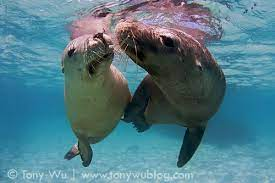
\includegraphics[width=0.7\textwidth]{sea_lions_holding_hands.jpg}
%DIFDELCMD < 	%%%
\DIFdelendFL \DIFaddbeginFL 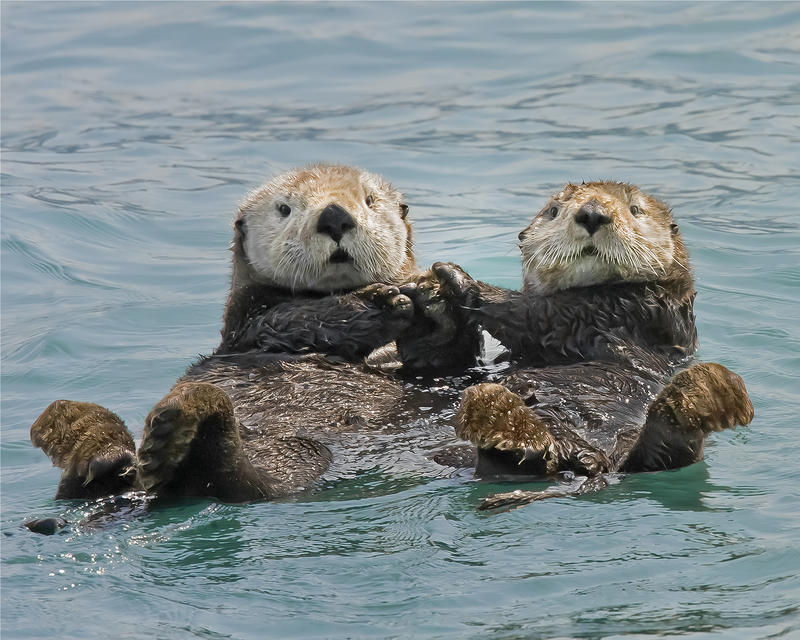
\includegraphics[width=0.7\textwidth]{sea_otters_holding_hands_by_ken_conger.jpg}
	\DIFaddendFL \caption{Sea \DIFdelbeginFL \DIFdelFL{Lions }\DIFdelendFL \DIFaddbeginFL \DIFaddFL{OTTURS }\DIFaddendFL Holding Hands}
	\label{fig:sealion}
\end{figure}

Here, \DIFdelbegin \DIFdel{sealions }\DIFdelend \DIFaddbegin \DIFadd{otturs }\DIFaddend are holding hands \ref{fig:sealion}

In the table, we can see that \DIFdelbegin \DIFdel{sealions }\DIFdelend \DIFaddbegin \DIFadd{seaotturs }\DIFaddend are simply superior
\begin{table}[H]
	\centering
	\begin{tabular}{||c c c c||} 
		\hline
		Fish & \DIFaddbeginFL \DIFaddFL{Sealions }& \DIFaddendFL Seaotturs & \DIFdelbeginFL \DIFdelFL{Sealion }%DIFDELCMD < & %%%
\DIFdelendFL Magic \\ [0.5ex] 
		\hline\hline
		1 & 6 & 87837 & $\omega$ \\ 
		2 & 7 & 78 & $\Omega$  \\
		3 & 545 & 778 & $\delta$  \\
		4 & 545 & 18744 & $\alpha$  \\
		5 & 88 & 788 & $\beta$  \\ [1ex] 
		\hline
	\end{tabular}
	\caption{Table to test captions and labels. \DIFdelbeginFL \DIFdelFL{\mbox{%DIFAUXCMD
\cite{Lions2001}}\hskip0pt%DIFAUXCMD
}\DIFdelendFL \DIFaddbeginFL \DIFaddFL{\mbox{%DIFAUXCMD
\cite{Otturs2020}}\hskip0pt%DIFAUXCMD
}\DIFaddendFL }
	\label{table:1}
\end{table}

\DIFaddbegin \DIFadd{And this table we can clearly see seaotturs just goign crazy
}

\DIFadd{In the table, we can see that seaotturs are simply superior
}\begin{table}[H]
	\centering
	\begin{tabular}{||c c c c||} 
		\hline
		\DIFaddFL{Fish }& \DIFaddFL{Sealions }& \DIFaddFL{Seaotturs }& \DIFaddFL{Magic }\\ 
		\hline\hline
		\DIFaddFL{1 }& \DIFaddFL{6 }& \DIFaddFL{$\infty$ }& \DIFaddFL{$\omega$ }\\ 
		\DIFaddFL{2 }& \DIFaddFL{7 }& \DIFaddFL{$\infty$ }& \DIFaddFL{$\Omega$  }\\
		\DIFaddFL{3 }& \DIFaddFL{545 }& \DIFaddFL{$\infty$ }& \DIFaddFL{$\delta$  }\\
		\DIFaddFL{4 }& \DIFaddFL{545 }& \DIFaddFL{$\infty$ }& \DIFaddFL{$\alpha$  }\\
		\DIFaddFL{5 }& \DIFaddFL{88 }& \DIFaddFL{$\infty$ }& \DIFaddFL{$\beta$  }\\
		\hline
	\end{tabular}
	\caption{\DIFaddFL{Table to test captions and labels. \mbox{%DIFAUXCMD
\cite{Otturs2020}}\hskip0pt%DIFAUXCMD
}}
	\label{table:2}
\end{table}

	\DIFaddend \bibliographystyle{unsrt}
	\begin{thebibliography}{1}

\DIFdelbegin \bibitem{Lions2001}
\DIFdel{Magical Sealions}\DIFdelend \DIFaddbegin \bibitem{Otturs2020}
\DIFadd{The Scientists}\DIFaddend .
\newblock \DIFdelbegin \DIFdel{Sealions rule.
}%DIFDELCMD < \newblock %%%
\DIFdelend {\em \DIFdelbegin \DIFdel{Under the water}\DIFdelend \DIFaddbegin \DIFadd{Seaotturs Truly rule}\DIFaddend }\DIFdelbegin \DIFdel{, page 217–244, 2001.
}\DIFdelend \DIFaddbegin \DIFadd{.
}\newblock \DIFadd{Penguins and Otturs, 3rd edition, 2019.
}\DIFaddend 

\end{thebibliography}

\end{document}